\documentclass[11pt]{article}
\usepackage{amsmath,amsthm,amsfonts}
\usepackage{tikz}
\usetikzlibrary{calc}
\usepackage{pgfplots}
\pgfplotsset{compat=newest}
\tikzset{
	pics/myrec/.style n args={3}{code={
			\draw[draw=none, #3] (0,0) rectangle (#1,#2);
	}},
	pics/myrec/.default={1}{0}{pink},
}
\usepackage{xcolor}

\begin{document}

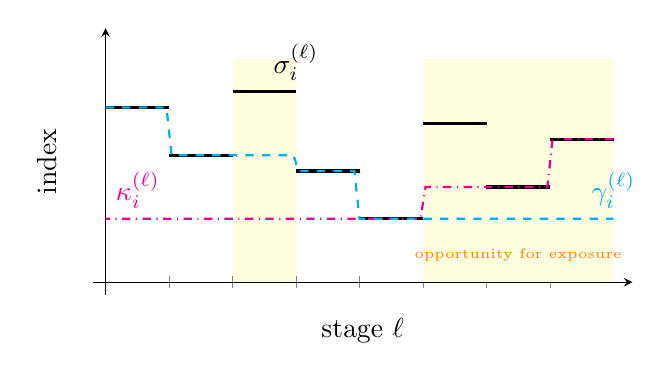
\begin{tikzpicture}[scale=1,domain=0:8,
	declare function={
		sig1(\x)= 2.75;
	},
	declare function={
		sig2(\x)= 2;
	},
	declare function={
		sig3(\x)= 3;
	},
	declare function={
		sig4(\x)= 1.75;
	},
	declare function={
		sig5(\x)= 1;
	},
	declare function={
		sig6(\x)= 2.5;
	},
	declare function={
		sig7(\x)= 1.5;
	},
	declare function={
		sig8(\x)= 2.25;
	},
	declare function={
		gamma(\x)= (\x < 1) * (2.75) +
		and(1 <= \x, \x < 3) * (2)  +
		and(3 <= \x, \x < 4) * (1.75)  +
		(4 <= \x) * (1)
	;
	},
	declare function={
	kappa(\x)= (\x < 5) * (1) +
	and(5 <= \x, \x < 7) * (1.5)  +
	(7 <= \x) * (2.25)
	;
	}
	]



	\begin{axis}[
		axis lines=middle,
		ymin=-0.2, ymax=4,
		xmin=-0.2, xmax=8.3,
		ymajorticks=false,
		xtick={0,...,7},
		y label style={at={(axis description cs:-0.05,0.5)},rotate=90,anchor=south},
		x label style={at={(axis description cs:0.5,-0.05)},anchor=north},
		ylabel=index,
		xlabel=stage $\ell$,
		xticklabel=\empty,
		domain=0:8,samples=101,
		axis equal image
		]


		\pic at (1.8,-.19) {myrec={1}{3.5}{fill=yellow!12.5!white}};
		\pic at (4.8,-.19) {myrec={3}{3.5}{fill=yellow!12.5!white}};

		\addplot [black,very thick,domain=0:1] {sig1(x)};
		\addplot [black,very thick,domain=1:2] {sig2(x)};
		\addplot [black,very thick,domain=2:3] {sig3(x)} node[above] {$\sigma_i^{(\ell)}$};
		\addplot [black,very thick,domain=3:4] {sig4(x)};
		\addplot [black,very thick,domain=4:5] {sig5(x)};
		\addplot [black,very thick,domain=5:6] {sig6(x)};
		\addplot [black,very thick,domain=6:7] {sig7(x)};
		\addplot [black,very thick,domain=7:8] {sig8(x)};


		\addplot [dashdotted, magenta, thick,domain=8:0] {kappa(x)} node[above right] {$\kappa_i^{(\ell)}$};

		\addplot [dashed, cyan, thick] {gamma(x)}  node[above] {$\gamma_i^{(\ell)}$};
	\end{axis}

\node [color=orange] at (5.4,0.5) {\tiny opportunity for exposure};

\end{tikzpicture}

\end{document}